%
% db-gleichverteilung.tex -- Datenblatt der stetigen gleichverteilung
%
% (c) 2015 Prof Dr Andreas Mueller, Hochschule Rapperswil
%
\subsection{Steckbrief}
\begin{center}
\begin{tabular}{|l|l|}
\hline
Name&Gleichverteilung\\
\hline
Dichtefunktion&
\begin{minipage}{3.7in}
\vskip5pt
$\displaystyle
\begin{cases}
\frac1{b-a}&\qquad a\le x\le b\\
0&\qquad\text{sonst}
\end{cases}
$
\end{minipage}
\\[8pt]
Verteilungsfunktion&
\begin{minipage}{3.7in}
\vskip5pt
$\displaystyle
\begin{cases}0&\qquad x\le a\\
\frac{x-a}{b-a}&\qquad x \le a \le b\\
1&\qquad x>b\end{cases}
$
\end{minipage}
\\[8pt]
Erwartungswert&
\begin{minipage}{3.7in}
\vskip3pt
$\displaystyle \frac{a+b}2$
\end{minipage}
\\[8pt]
Varianz&
\begin{minipage}{3.7in}
\vskip3pt
$\displaystyle \frac{(b-a)^2}{12}$
\end{minipage}
\\[8pt]
Median&
\begin{minipage}{3.7in}
\vskip3pt
$\displaystyle \frac{a+b}{2}$
\end{minipage}
\\[8pt]
$P(|X-E(X)|>\varepsilon)$&
\begin{minipage}{3.7in}
\vskip3pt
$\displaystyle 1-\frac{2\varepsilon}{b-a}$ für $\varepsilon<\frac{b-a}2$
\end{minipage}
\\[10pt]
\hline
Anwendungen&\begin{minipage}{3.7in}%
\strut
$\bullet$ Verteilung von Zufallszahlen
\strut
\\
\strut
$\bullet$ Keine bevorzugten Werte
\strut
\end{minipage}\\
\hline
\end{tabular}
\end{center}

\subsection{Verteilungsfunktion und Wahrscheinlichkeitsdichte}
Verteilungsfunktion (oben) und Wahrscheinlichkeitsdichte (unten)
der Gleichverteilung:
\begin{center}
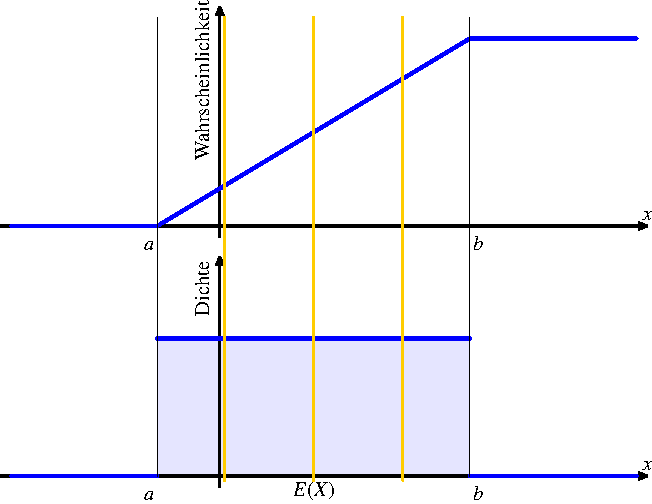
\includegraphics[width=0.8\hsize]{images/verteilungsfunktion-7}
\end{center}

\subsection{Wahrscheinlichkeit einer grossen Abweichung}
Wahrscheinlichkeit einer Abweichung vom Mittelwert einer
in $[0,1]$ gleichverteilten Zufallsvariable (rot) im Vergleich mit
der oberen Schranke aus dem Satz von Tschebyscheff (grün):
\begin{center}
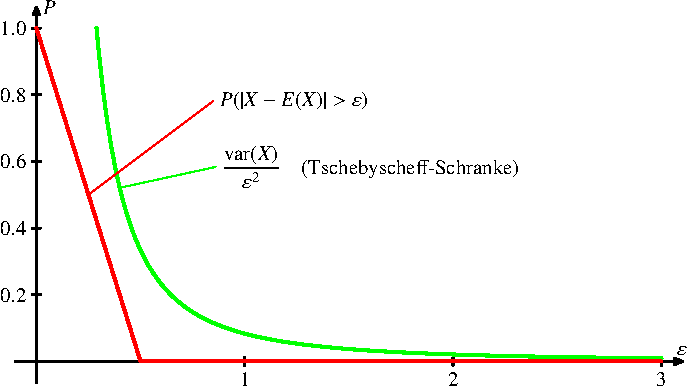
\includegraphics{images/gl-1.pdf}
\end{center}

\subsection{Parameter schätzen}
Die Parameter $a$ und $b$ der Gleichverteilung können mit den 
erwartungstreuen Schätzern
\begin{align*}
\hat a(x_1,\dots,x_n)=\frac{n+1}{n}\min(x_1,\dots,x_n)\\
\hat b(x_1,\dots,x_n)=\frac{n+1}{n}\max(x_1,\dots,x_n)
\end{align*}
geschätzt werden.
